\section{Density Functional Theory}




\subsection{Quantum Espresso}







Degauss values 0.01Ry Methessel-Paxton \cite{AdsorptionBR2}
Fermi-Dirac 0.01eV (0.00074Ry) \cite{NaDiffusion}
Marzari-Vanderbilt 0.01Ry \cite{ScBiandYBi}
Degauss 0.03 + 0.05 \cite{CuandPd}
Marzari-Vanderbilt 0.05Ry \cite{ecHeuslerAlloy}




\subsection{Crystal Structure}


A large amount of computing power is required to run the DFT calculations.  If the input parameters are not accurate enough to begin with, it will either take a long time for the DFT calculation to run, or it will fail to converge completely.


\begin{table}[h]
\begin{center}
\begin{tabular}{c c c c c c}
\hline
Element & Atomic Mass & Density kg/m\textsuperscript{3} & Atoms/m\textsuperscript{3} & FCC (Bohr/Angstrom) & BCC (Bohr/Angstrom) \\
\hline
Al     & 26.98  &  2700   &  $6.02 \times 10^{28}$    & 7.66/4.05    & 6.08/3.22   \\ 
Fe     & 55.84  &  7874   &  $8.47 \times 10^{28}$    & 6.83/3.61    & 5.42/2.87   \\ 
Pd     & 106.42 &  12023  &  $6.83 \times 10^{28}$    & 7.34/3.88    & 5.83/3.08   \\ 
Ni     & 58.69  &  8908   &  $9.09 \times 10^{28}$    & 6.67/3.53    & 5.30/2.80   \\ 
\end{tabular}
\end{center}
\caption{Predicted lattice parameters based on the density, atomic number and type of structure}
\end{table}





\subsection{Pseudopotential Selection}

The pseudopotentials were downloaded from the Quantum Espresso PSLibrary with url:

http://www.quantum-espresso.org/pseudopotentials/pslibrary 

There are several categories of pseudopotential available.  The pseudopotentials may be fully relativistic or not.  The DFT calculations will be collinear or no spin calculations, and the element with the largest number of electrons will be Palladium, with electrons in the s, p, d shells.  There will be no elements used in this work with f shell electrons, so a non-relativistic pseudopoential will be used for each element.

There are a number of choices of exchange-correlation functional, depending on the element:

\begin{itemize}
\item pz: Perdew-Zunger (LDA)
\item vwn: Vosko-Wilk-Nusair (LDA)
\item pbe: Perdew-Burke-Ernzerhof (GGA)
\item blyp: Becke-Lee-Yang-Parr (BLYP)
\item pw91: Perdew-Wang 91 gradient-corrected 
\end{itemize}

In the literature, LDA and BLYP are used for organic DFT calculations.  LDA and GGA type pseudopotentials have been used to model solids and, in particular, the GGA type have been used to study metals as they are more reliable at calculating parameters such as $a_0$.

Several elements were tested to compare the results of LDA and GGA pseudopotentials to the experimental values for the lattice parameter of each.

The settings used were:

\begin{itemize}
\item ecutwfc: 71 
\item ecutrho: 430 
\item k-points: 9 9 9 Monhurst-Pack grid offset
\item smearing: 0.04 Ry Mazari-Vanderbilt cold smearing
\item calculation type: non-polarised calculation
\item pseudopotentials: PZ for LDA, PBE for GGA
\end{itemize}

The results were computed as follows:

\begin{table}[h]
\begin{center}
\begin{tabular}{c c c c c}
\hline
Element & Crystal & $a_0$ exp. (ang) & $a_0$ LDA (ang) & $a_0$ GGA (ang) \\
\hline
Al     & FCC  &  4.05  &  3.98  &  4.04   \\ 
Fe     & BCC  &  2.87  &  2.69  &  2.75   \\ 
Pd     & FCC  &  3.89  &  3.84  &  3.93   \\ 
Cu     & FCC  &  3.61  &  3.49  &  3.59   \\ 
\end{tabular}
\end{center}
\caption{Predicted lattice parameters based on the density, atomic number and type of structure}
\end{table}

The simpler LDA pseudopotentials consistently underestimate the lattice parameter $a_0$ for the four metals tested, and on average they underestimate by 3%.  The GGA calculations are within 1.5% of the experimental value 



\subsection{Qeconverge Python Program}

The process of converging cutoff parameters is one that may be automated.  A program was written in Python to automatically converge the ecutwfc and ecutrho values within a specified threshold.

The program reads an input file into memory, and this contains the settings for the convergence run.  A template PWscf input file is also loaded, and this will have any required PWscf settings, such as the pseudopotentials, atom species and so on.  

Once these files have been loaded, the first stage of the program runs to determine the ecutwfc and ecutrho values that are within the force and energy convergence thresholds.  The program creates a crystal based on the settings, for example an FCC, BCC or SC crystal supercell.  The exact atomic positions are likely to be the optimal, relaxed, positions and so the overall forces on each atom will be zero.  The program randomly varies the atomic positions, and this results in a configuration with forces between the atoms.

The wfc value starts with the user defined ecutwfc starting value, and this is increased until the change in energy and force both converge to within the specified thresholds.  The ecutrho value is increased simultaneously, and is four times the ecutwfc value.  In the second stage, the ecutrho value is decreased and the ecutwfc value is held constant while the energy and force remain within their respective convergence thresholds.  Finally, the program attempts to decrease the ecutwfc value further.

Following the energy and charge density cutoff, the program then runs a number of calculations in order to produce a number of colour density plots of energy cutoff vs density cutoff, plotting the convergence of total energy and total force.  This allows the user to visualise the convergence surface and select cutoff values manually.

\begin{center}
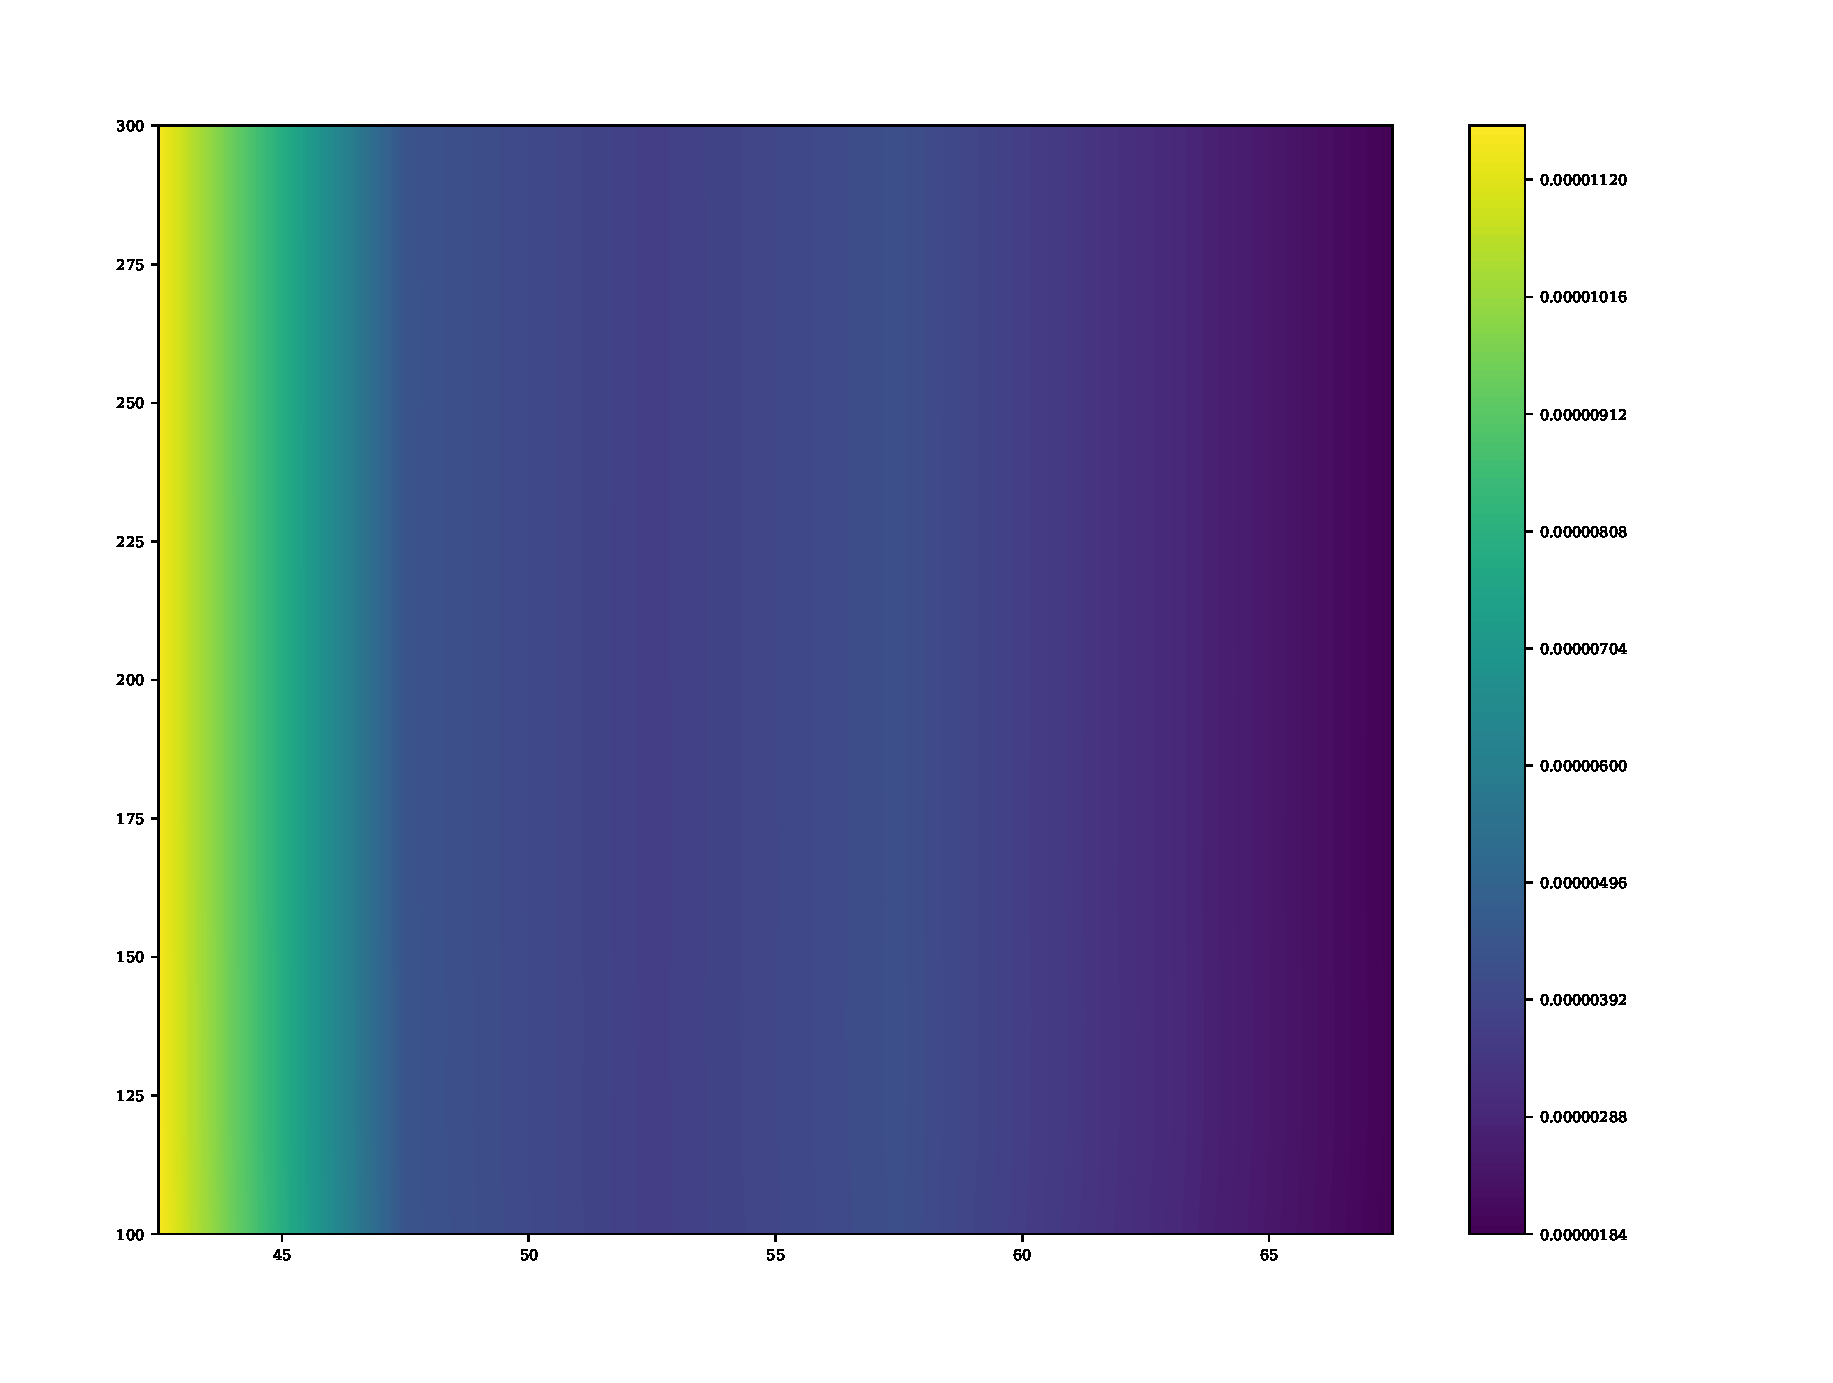
\includegraphics[scale=0.35]{chapters/methodology_interatomic_potentials/qeconverge/ecut2d_energy_wfcconv_ry_colour}
\end{center}

The final part of the program is to help the user decide upon degauss and k-point values.  The converged ecutwfc and ecutrho values from the first part of the code are used, and the k-point start, end and increment amounts are set by the user, as is a list of smearing degauss values.  2D colour plots of force and energy convergence as smearing changes and k-point value changes are prepared and saved so the user may study these to determine the best combination for their application.

\begin{center}
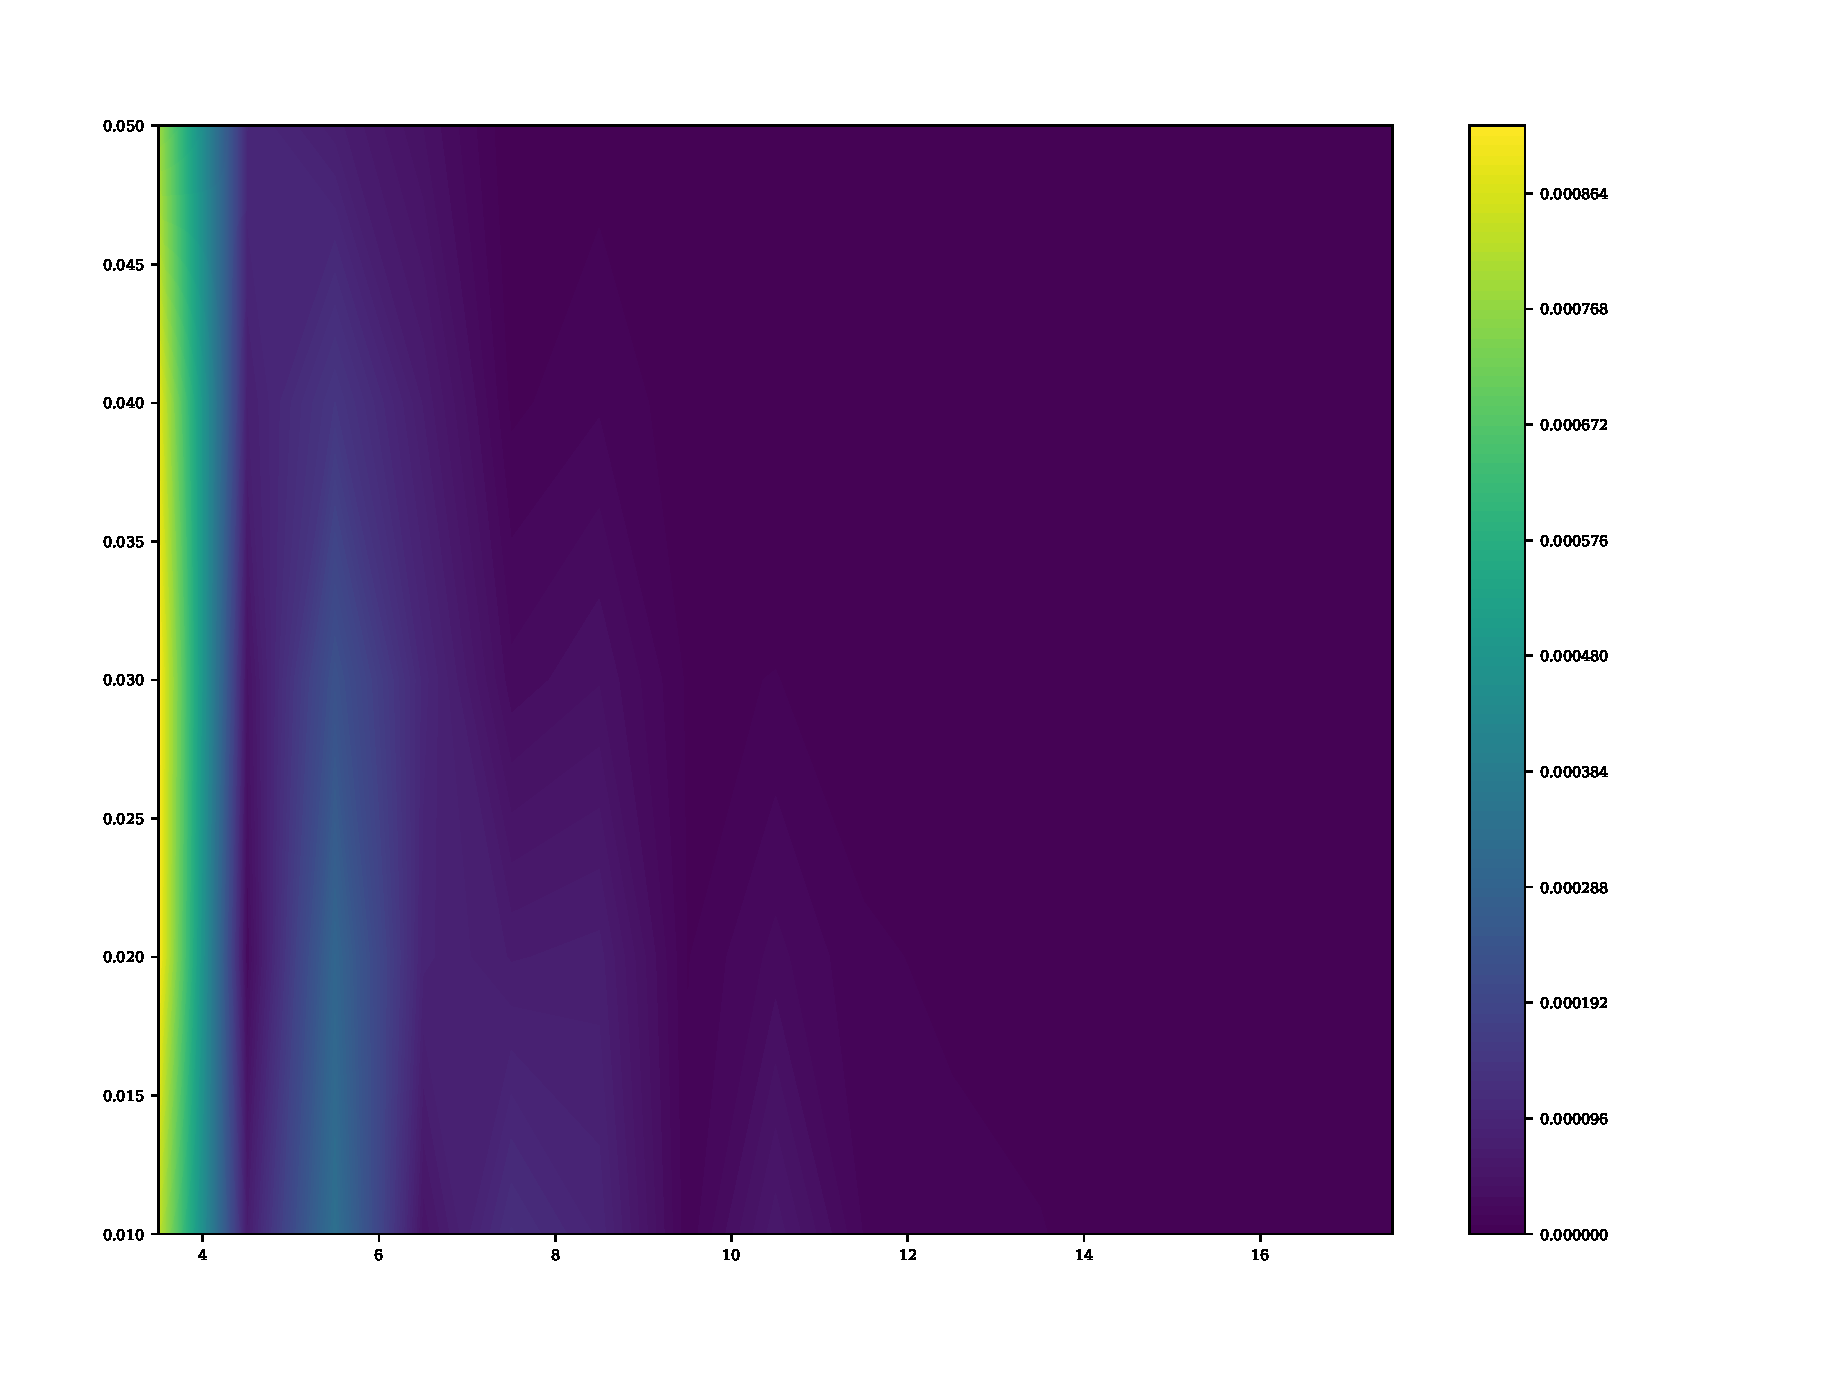
\includegraphics[scale=0.35]{chapters/methodology_interatomic_potentials/qeconverge/kpoints_energy_kpointconv_ry_colour}
\end{center}

The randomised atom positions use a seed that may be set in the input file.  This means that, although they are pseudo-rng generated, they are repeatable given the same random seed.  Every successful PWscf calculation is logged and saved, and if the program runs multiple times, the cached output files are used rather than recalculating every input file.















